\chapter{Future Work}
As of the composing this document, the project is still in prototype stage. This project is meant to produce an easy to use experiment automation software. 
\section{Functionality To Be Added}

\subsection{Behaviour Analysis}

This software will provide users all data such as: 
\begin{itemize}
\item mean of position
\item standard deviation of position
\item position history
\item active time periods
\item inactive time periods
\item areas highly frequented by the subject animal
\end{itemize}
and any other report our product owners may require.

\subsection{Experiment Setup}
We will implement a "New Experiment" Wizard which will guide the end-user through creation of automated experiments. 

Default parameters for the Wizard will be determined to make this process as streamlined as possible.

\subsection{Performance Improvements}
Currently the system is working with 30fps framerate which gives us roughly 33 ms to track objects, log data and record the processed video. As of the project midterm the program is a bir resource heavy and works with occasional lag. 

We will reduce runtime load by running object tracking on image pyramids instead of raw data.

By using image pyramids we will first determine rough locations of objects on a much lower resolution image and work our way up for parts that seem to contain objects. Thus relieving the system of unnecessary load of scanning empty areas in high resolution.

\subsection{Offline experiments}
One of the functionalities we aim to implement is running the same experiment off-line at a later time.This functionality is essential since this product is meant for scientific purposes which require a certain degree of repeatability.

By providing the user with off-line experiments any user can check and validate another's experiment which brings credibility to experiments.

\subsection{Exploring Kinect 2}
In early 2014 Microsoft released its successor to Kinect, Kinect 2 which has much higher resolution output and very high performance as shown in figure \ref{fig:KK2}.
\begin{figure}
    \centering
    \subfloat[Kinect]{{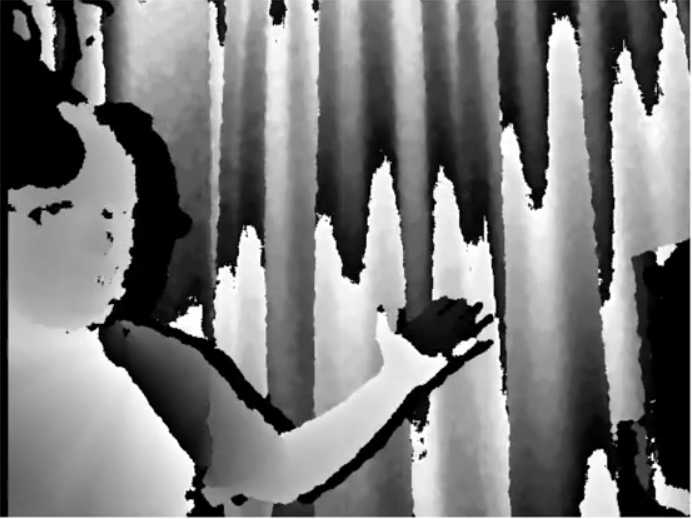
\includegraphics[scale=0.75]{./K1}}}%
    \qquad
    \subfloat[Kinect 2]{{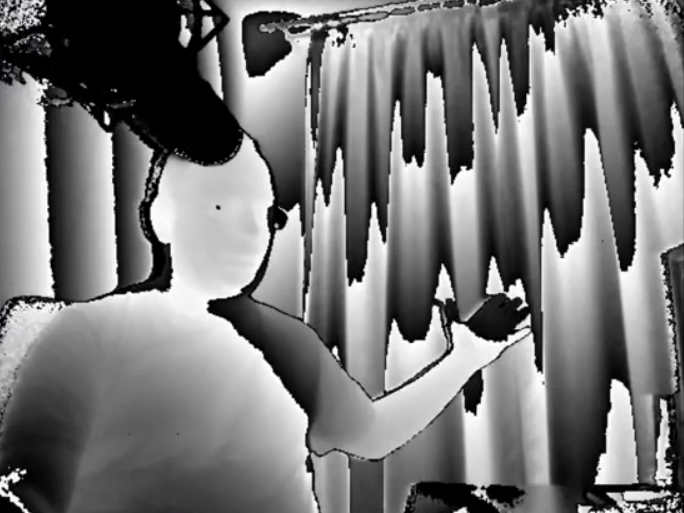
\includegraphics[scale=0.75]{./K2}}}%
    \caption{Kinect Output vs Kinect 2 Output}
    \label{fig:KK2}
\end{figure}

We will explore Kinect 2 as a new sensor. If the extra resolution doesn't hit performance too hard we will consider switching to it to be able to work with much cleaner data. 